\documentclass[tikz]{standalone}

\usetikzlibrary{shapes}

\begin{document}

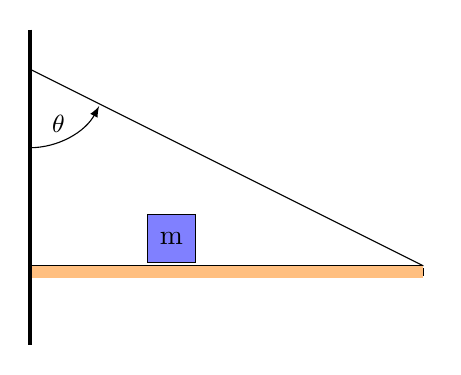
\begin{tikzpicture}
    \draw (0,0)-- (5,0) node (a){};
    \draw (0,-0.15)-- (5,-0.15) node (b){};
    \draw (0,2.5) -- (5,0);
    \draw[-latex] (0,1.5) arc (-90:-28:1) node[midway,label={[shift={(-0.15,-0.2)}]\small{$\theta$}}] {};
    \fill [orange!50] (0,0) rectangle (5,-0.15) ;
    \draw (a)--(b);
    \node at (1.8,0.35) [regular polygon,regular polygon sides=4,draw,inner sep=2,fill=blue!50]{m};
    \draw[line width=0.5mm] (0,3)--(0,-1);
\end{tikzpicture}

\end{document}